%\documentclass[landscape,a0b,final,a4resizeable]{a0poster}
\documentclass[landscape,a0b,final]{a0poster}
%\documentclass[portrait,a0b,final,a4resizeable]{a0poster}
%\documentclass[portrait,a0b,final]{a0poster}
%%% Option "a4resizeable" makes it possible ot resize the
%   poster by the command: psresize -pa4 poster.ps poster-a4.ps
%   For final printing, please remove option "a4resizeable" !!

\usepackage{epsfig}
\usepackage{multicol}
\usepackage{cite}
\usepackage[font=footnotesize]{subfig}
\usepackage{float}
\usepackage{setspace}
\usepackage{amsmath, amssymb, bm}
\DeclareMathOperator*{\argmin}{arg\,min}
\onehalfspacing
\usepackage{mathtools}
\usepackage{pstricks,pst-grad}

%%%%%%%%%%%%%%%%%%%%%%%%%%%%%%%%%%%%%%%%%%%
% Definition of some variables and colors
%\renewcommand{\rho}{\varrho}
%\renewcommand{\phi}{\varphi}
\setlength{\columnsep}{.5cm}
\setlength{\columnseprule}{2mm}
\setlength{\parindent}{0.0cm}



%%%%%%%%%%%%%%%%%%%%%%%%%%%%%%%%%%%%%%%%%%%%%%%%%%%%
%%%               Background                     %%%
%%%%%%%%%%%%%%%%%%%%%%%%%%%%%%%%%%%%%%%%%%%%%%%%%%%%

\newcommand{\background}[3]{
  \newrgbcolor{cgradbegin}{#1}
  \newrgbcolor{cgradend}{#2}
  \psframe[fillstyle=gradient,gradend=cgradend,
  gradbegin=cgradbegin,gradmidpoint=#3](0.,0.)(1.\textwidth,-1.\textheight)
}



%%%%%%%%%%%%%%%%%%%%%%%%%%%%%%%%%%%%%%%%%%%%%%%%%%%%
%%%                Poster                        %%%
%%%%%%%%%%%%%%%%%%%%%%%%%%%%%%%%%%%%%%%%%%%%%%%%%%%%

\newenvironment{poster}{
  \begin{center}
  \begin{minipage}[c]{0.98\textwidth}
}{
  \end{minipage}
  \end{center}
}



%%%%%%%%%%%%%%%%%%%%%%%%%%%%%%%%%%%%%%%%%%%%%%%%%%%%
%%%                pcolumn                       %%%
%%%%%%%%%%%%%%%%%%%%%%%%%%%%%%%%%%%%%%%%%%%%%%%%%%%%

\newenvironment{pcolumn}[1]{
  \begin{minipage}{#1\textwidth}
  \begin{center}
}{
  \end{center}
  \end{minipage}
}



%%%%%%%%%%%%%%%%%%%%%%%%%%%%%%%%%%%%%%%%%%%%%%%%%%%%
%%%                pbox                          %%%
%%%%%%%%%%%%%%%%%%%%%%%%%%%%%%%%%%%%%%%%%%%%%%%%%%%%

\newrgbcolor{lcolor}{0. 0. 0.80}
\newrgbcolor{gcolor1}{1. 1. 1.}
\newrgbcolor{gcolor2}{.80 .80 1.}

\newcommand{\pbox}[4]{
\psshadowbox[#3]{
\begin{minipage}[t][#2][t]{#1}
#4
\end{minipage}
}}



%%%%%%%%%%%%%%%%%%%%%%%%%%%%%%%%%%%%%%%%%%%%%%%%%%%%
%%%                myfig                         %%%
%%%%%%%%%%%%%%%%%%%%%%%%%%%%%%%%%%%%%%%%%%%%%%%%%%%%
% \myfig - replacement for \figure
% necessary, since in multicol-environment
% \figure won't work

\newcommand{\myfig}[3][0]{
\begin{center}
  \vspace{1.5cm}
  \includegraphics[width=#3\hsize,angle=#1]{#2}
  \nobreak\medskip
\end{center}}



%%%%%%%%%%%%%%%%%%%%%%%%%%%%%%%%%%%%%%%%%%%%%%%%%%%%
%%%                mycaption                     %%%
%%%%%%%%%%%%%%%%%%%%%%%%%%%%%%%%%%%%%%%%%%%%%%%%%%%%
% \mycaption - replacement for \caption
% necessary, since in multicol-environment \figure and
% therefore \caption won't work

%\newcounter{figure}
\setcounter{figure}{1}
\newcommand{\mycaption}[1]{
  \vspace{0.5cm}
  \begin{quote}
    {{\sc Figure} \arabic{figure}: #1}
  \end{quote}
  \vspace{1cm}
  \stepcounter{figure}
}



%%%%%%%%%%%%%%%%%%%%%%%%%%%%%%%%%%%%%%%%%%%%%%%%%%%%%%%%%%%%%%%%%%%%%%
%%% Begin of Document
%%%%%%%%%%%%%%%%%%%%%%%%%%%%%%%%%%%%%%%%%%%%%%%%%%%%%%%%%%%%%%%%%%%%%%

\begin{document}

\background{1. 1. 1.}{1. 1. 1.}{0.5}


\newrgbcolor{lightblue}{0. 0. 0.80}
\newrgbcolor{white}{1. 1. 1.}
\newrgbcolor{whiteblue}{.80 .80 1.}


\begin{poster}

%%%%%%%%%%%%%%%%%%%%%
%%% Header
%%%%%%%%%%%%%%%%%%%%%
\begin{center}
\begin{pcolumn}{1}

\pbox{0.98\textwidth}{}{linewidth=2mm,framearc=0.3,linecolor=lightblue,fillstyle=gradient,gradangle=0,gradbegin=white,gradend=whiteblue,gradmidpoint=1.0,framesep=1em}{

%%% Unisiegel
\begin{minipage}[c][9cm][c]{0.1\textwidth}
  \begin{center}
    %\includegraphics[width=7cm,angle=0]{}
  \end{center}
\end{minipage}
%%% Titel
\begin{minipage}[c][16cm][c]{0.78\textwidth}
  \begin{center}
      {\sc \Huge \textbf{A PSF photometry tool for NASA's Kepler,} $\mathcal{K}\mathbf{2}$\textbf{, and TESS missions}}\\[7mm]
      {\Large \textbf{Jos\'e Vin\'icius de Miranda Cardoso}$^{1, 2, 4}$, \textbf{Geert Barentsen}$^{1, 2}$,
       \textbf{Ben Montet}$^{3, \bm{\star}}$,}\\
      {\Large \textbf{Ann Marie Cody}$^{1, 2}$,
       \textbf{Christina Hedges}$^{1, 2}$ and \textbf{Michael Gully-Santiago}$^{1, 2}$}\\
      {\Large $^{1}$NASA Ames Research Center, Moutain View, CA, USA\\
       $^{2}$Bay Area Environmental Research Institute, Petaluma, CA, USA\\
       $^{3}$Department of Astrophysics, University of Chicago, IL, USA\\
       $^{4}$Federal University of Campina Grande, Campina Grande, Brazil\\
       $^{\bm{\star}}$NASA Sagan Fellow}
  \end{center}
\end{minipage}
%%% GK-Logo
\begin{minipage}[c][9cm][c]{0.1\textwidth}
  \begin{center}
    %\includegraphics[width=7cm,angle=0]{}
  \end{center}
\end{minipage}

}
\end{pcolumn}
\end{center}

\vspace*{.5cm}

%%%%%%%%%%%%%%%%%%%%%
%%% Content
%%%%%%%%%%%%%%%%%%%%%
\begin{center}
\begin{pcolumn}{0.32}
\pbox{0.90\textwidth}{65cm}{linewidth=2mm,framearc=0.1,linecolor=lightblue,fillstyle=gradient,gradangle=0,gradbegin=white,gradend=white,gradmidpoint=1.0,framesep=1em}{

\begin{center}\pbox{0.8\textwidth}{}{linewidth=2mm,framearc=0.1,linecolor=lightblue,fillstyle=gradient,gradangle=0,gradbegin=white,gradend=whiteblue,gradmidpoint=1.0,framesep=1em}{\begin{center}\textbf{Introduction}\end{center}}\end{center}
\vspace{0.75cm}

\begin{itemize}
    \item NASA's Kepler and K2 missions have been delivering high-precision time series data for a wide range of stellar types
    \item However, both the official and community developed pipelines~\cite{luger, vanderburg, aigrain} tend to focus on studying
          isolated stars using simple aperture photometry, hence performing sub-optimally in crowded fields
    \item Although Point Spread Function (PSF) photometry methods are well
          known~\cite{anderson, libralato1}, as of now, there exist
          no open source tool that takes into account the caveats inherent in Kepler and $\mathcal{K}$2 data
    \item To address this issue, we present an open source PSF photometry toolkit for Kepler and K2
        and extensible to TESS, as part of the $\mathcal{K}2$ Guest Obverser Office data analysis tool, PyKE
\end{itemize}

\vspace{0.75cm}
\begin{center}\pbox{0.8\textwidth}{}{linewidth=2mm,framearc=0.1,linecolor=lightblue,fillstyle=gradient,gradangle=0,gradbegin=white,gradend=whiteblue,gradmidpoint=1.0,framesep=1em}{\begin{center}\textbf{Methods}\end{center}}\end{center}
\vspace{0.75cm}

    \begin{center}
        \textbf{Fitting multiple PSFs jointly}
    \end{center}

    Consider an experiment that outputs an image with $m$ ($m$ known) stellar objects as a collection of $n$ independent \emph{non-identically} distributed random variables $\bm{Y} \triangleq \{Y_i\}_{i=1}^{n}$ (pixels), each of which has expected value $\mathbb{E}\left[Y_i\right] = \sum_{j=1}^{m}\lambda_i(\bm{\Theta}_j)$, where $\lambda_i$ is the PSF model at the $i$-th pixel, $\bm{\Theta}_j$ is a random vector
    that encondes the information about flux and center position of the $j$-th star. Hence, the likelihood function can be
    written as
\begin{align}
   P\left(\bm{Y} = \bm{y} \Bigr| \left\{\bm{\Theta}_j\right\}_{j=1}^{m} = \left\{\bm{\theta}_j\right\}_{j=1}^{m}\right) = \exp\left({-\sum_{i=1}^{n}\sum_{j=1}^{m}\lambda_i(\bm{\theta}_j)}\right)\prod_{i=1}^{n}\dfrac{\left(\sum_{j=1}^{m}\lambda_i\left(\bm{\theta}_j\right)\right)^{y_i}}{y_i!}.
\end{align}

Perhaps of more practical interest is the log likelihood function
\begin{equation}
    \log  P\left(\bm{Y} = \bm{y} \Bigr| \left\{\bm{\Theta}_j\right\}_{j=1}^{m} = \left\{\bm{\theta}_j\right\}_{j=1}^{m}\right) = \sum_{i=1}^{n}\left(- \sum_{j=1}^{m}\lambda_i(\bm{\theta}_j) + y_i\log\sum_{j=1}^{m}\lambda_i(\bm{\theta}_j)\right).
\end{equation}

    Hence, the Maximum Likelihood Estimator (MLE) can be formulated as the following optimization problem
\begin{align}
    \bm{\theta}^{*}(\bm{y}) = \argmin_{\bm{\theta} \in \Lambda} \sum_{i=1}^{n}\left(\sum_{j=1}^{m}\lambda_i(\bm{\theta}_j) - y_i\log\sum_{j=1}^{m}\lambda_i(\bm{\theta}_j)\right).
\end{align}
Furthermore, prior probability densities (often taken to be uniform on $\Lambda$) on the stars positions, fluxes, and
sky background, are used.

\vspace{0.75cm}
    \begin{center}
        \textbf{Estimating uncertainties using the Cram\'er-Rao Lower Bound}
    \end{center}

Uncertainties on the fitted values are computed using the Cram\'er-Rao Lower Bound. Mathematically,
        \begin{equation}
            cov(\bm{\theta}^{*}(\bm{Y})) \leq \left(\mathbb{E}_{\bm{\theta}}\left[\nabla_{\bm{\theta}}\log p(\bm{Y} | \bm{\theta})\left[\nabla_{\bm{\theta}}\log p(\bm{Y} | \bm{\theta}) \right]^{T}  \right]\right)^{-1}\Bigr|_{\substack{\bm{\theta}=\bm{\theta}^{*}(\bm{y})}}
        \end{equation}

}
\end{pcolumn}
\begin{pcolumn}{0.32}
\pbox{0.90\textwidth}{65cm}{linewidth=2mm,framearc=0.1,linecolor=lightblue,fillstyle=gradient,gradangle=0,gradbegin=white,gradend=white,gradmidpoint=1.0,framesep=1em}{


    \begin{center}
        \textbf{The Kepler Pixel Response Function Model}
        \begin{itemize}
            \item Kepler's pixel response function (PRF) has been shown to be nonsymmetric and spatially variant
                accross the detector~\cite{bryson}
            \item The PRF model used in PyKE is constructed following a similar procedure as stated by
                Bryson \textit{et al.}~\cite{bryson}
        \end{itemize}

        \includegraphics[width=15cm,angle=0]{figs/prf.eps}
        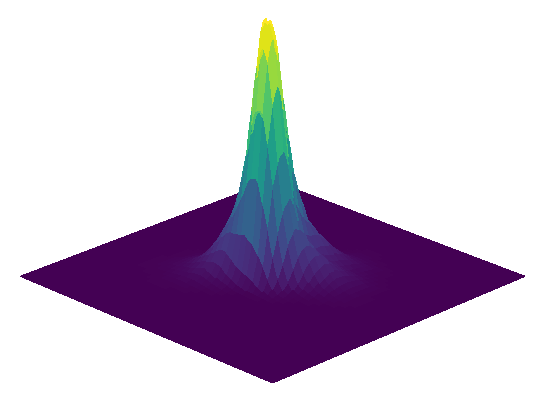
\includegraphics[width=16.5cm,angle=0]{figs/prf-deg-45.eps}

    \end{center}
            An object of the PSF model can be instantied as follows\\
        \texttt{>>> from pyke import KeplerTargetPixelFile} \\
        \texttt{>>> tpf = KeplerTargetPixelFile("ADDRESS\_TO\_TPF")}\\
        \texttt{>>> prf = tpf.get\_prf\_model()}

%%% Section
        \vspace{1.25cm}
\begin{center}\pbox{0.8\textwidth}{}{linewidth=2mm,framearc=0.1,linecolor=lightblue,fillstyle=gradient,gradangle=0,gradbegin=white,gradend=whiteblue,gradmidpoint=1.0,framesep=1em}{\begin{center}\textbf{Crowded K2 Clusters}\end{center}}\end{center}\vspace{1.25cm}

    \includegraphics[width=16cm,angle=0]{figs/tpf_c9.eps}
    \includegraphics[width=16cm,angle=0]{figs/model_c9.eps}
    \includegraphics[width=16cm,angle=0]{figs/residuals_c9.eps}
    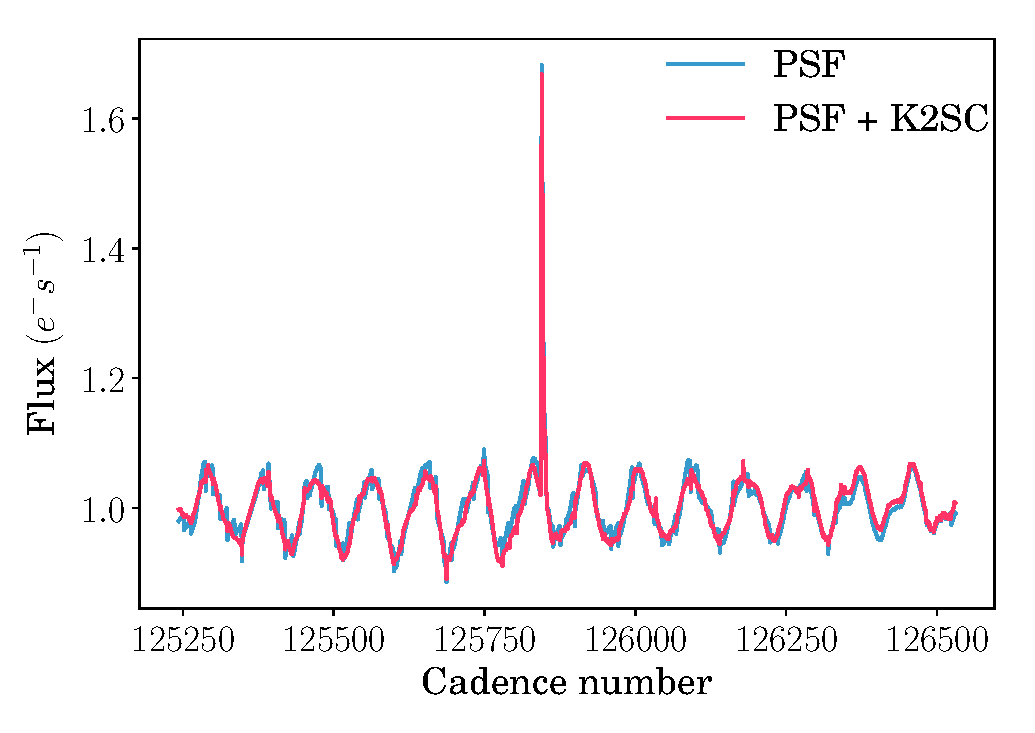
\includegraphics[width=17cm,angle=0]{figs/lc_c9.eps}

    \texttt{>>> from pyke.prf import SceneModel, PRFPhotometry}\\
    \texttt{>>> scene = SceneModel(prfs=5*[prf])} \\
    \texttt{>>> phot = PRFPhotometry(prior=prior, scene\_model=scene)} \\
    \texttt{>>> results = phot.fit(tpf.flux)} \\
}


\end{pcolumn}
\begin{pcolumn}{0.32}
\pbox{0.90\textwidth}{65cm}{linewidth=2mm,framearc=0.1,linecolor=lightblue,fillstyle=gradient,gradangle=0,gradbegin=white,gradend=white,gradmidpoint=1.0,framesep=1em}{

\begin{center}\pbox{0.8\textwidth}{}{linewidth=2mm,framearc=0.1,linecolor=lightblue,fillstyle=gradient,gradangle=0,gradbegin=white,gradend=whiteblue,gradmidpoint=1.0,framesep=1em}{\begin{center}\textbf{Kepler Faint Stars}\end{center}}\end{center}
\vspace{.5cm}

\includegraphics[width=16cm,angle=0]{figs/tpf_kep.eps}
    \includegraphics[width=16cm,angle=0]{figs/model_kep.eps}
    \includegraphics[width=16cm,angle=0]{figs/residuals_kep.eps}
    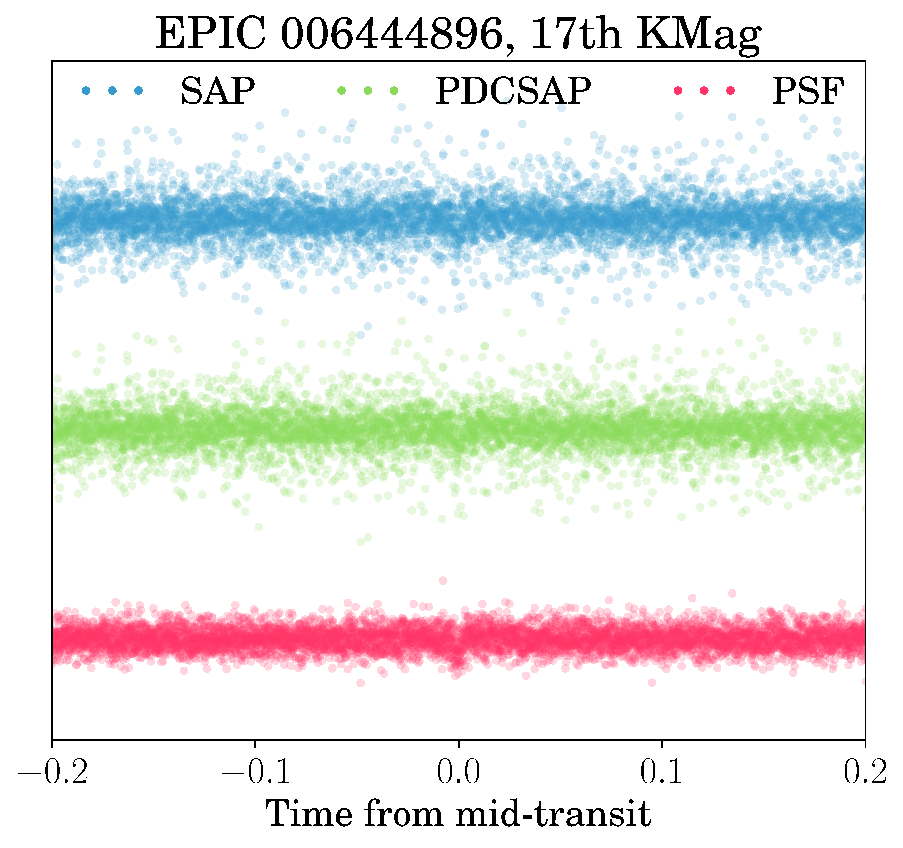
\includegraphics[width=16cm,angle=0]{figs/faint.eps}

\begin{center}\pbox{0.8\textwidth}{}{linewidth=2mm,framearc=0.1,linecolor=lightblue,fillstyle=gradient,gradangle=0,gradbegin=white,gradend=whiteblue,gradmidpoint=1.0,framesep=1em}{\begin{center}\textbf{Conclusions}\end{center}}\end{center}
\vspace{.5cm}

    \begin{itemize}
        \item We have presented an open-source tool to perform PSF photometry on Kepler and $\mathcal{K}$2 data
            which precisely and accurately estimates stellar positions and fluxes on the CCD
        \item Motion-dependent noise, primarily caused by the subpixel flat-field variations, which are not
            taken into account in the PSF model, is still present. Nevertheless, it can be easily removed
            by the procedures developed by detrending pipelines
        \item As future works, we intend to study novel ways to build the PSF model, especially by using
            data-driven approaches
    \end{itemize}

%%% References
\bibliographystyle{unsrt}
\bibliography{poster.bib}

}
\end{pcolumn}
\end{center}

\end{poster}

\end{document}

